%! Author = Len Washington III
%! Date = 1/17/24

% Preamble
\documentclass[title={Chapter 1}]{fdsn201notes}
\usepackage{textcomp}

% Packages

% Document
\begin{document}

\maketitle
\setcounter{chapter}{1}

\definecolor{healthpink}{HTML}{ff4c68}
\definecolor{healthgreen}{HTML}{95c82e}
\definecolor{healthblue}{HTML}{1869c3}
\definecolor{healthpurple}{HTML}{c855a5}
\definecolor{healthorange}{HTML}{e97610}

\definecolor{rowlightgreen}{HTML}{ffffef}
\definecolor{rowmedgreen}{HTML}{faffbf}
\definecolor{rowdarkgreen}{HTML}{d3df37}

\definecolor{nutrientgreen}{HTML}{3ead44}
\definecolor{nutrientorange}{HTML}{ff9607}
\definecolor{nutrientpink}{HTML}{d8809a}
\definecolor{nutrientred}{HTML}{ff2426}
\definecolor{nutrientpurple}{HTML}{536eb2}
\definecolor{nutrientblue}{HTML}{1581cc}

\section{What is Nutrition?}\label{sec:what-is-nutrition?}

\begin{itemize}
	\item \definition{Nutrition}{the study of food, including}
	\begin{itemize}
		\item How food nourished our bodies
		\item How food influences our health
	\end{itemize}
	\item Nutrition is a relatively new discipline of science.
	\item Nutrition research focuses on supporting health and preventing and/or treating chronic diseases.
	\item Nutrition involves study of the following:
	\begin{itemize}
		\item Food consumption
		\item Food digestion
		\item Food absorption
		\item Food storage
		\item Factors that influence eating patterns
		\item Recommended amounts of types of food
		\item Food safety
		\item The global food supply
	\end{itemize}
\end{itemize}

\section{How Does Nutrition Support Health?}\label{sec:how-does-nutrition-support-health?}
\begin{itemize}
	\item Nutrition supports health and wellness
	\item \definition{Wellness}{A multidimensional, active process by which people make choices to enhance their lives}
	\begin{itemize}
		\item Includes: physical, emotional, social, occupational, and spiritual health
	\end{itemize}
	\item Critical components of wellness
	\begin{itemize}
		\item Nutrition
		\item Physical activity
	\end{itemize}
\end{itemize}

\section{Wellness}\label{sec:wellness}
\textcolor{healthpink}{\subsection{Physical Health}\label{subsec:physical-health}}
Includes nutrition and physical activity.
%
\textcolor{healthgreen}{\subsection{Spiritual Health}\label{subsec:spiritual-health}}
Includes spiritual values and beliefs.
%
\textcolor{healthblue}{\subsection{Emotional Health}\label{subsec:emotional-health}}
Includes positive feelings about one's self and life.
%
\textcolor{healthpurple}{\subsection{Social Health}\label{subsec:social-health}}
Includes family, community, and social environment.
%
\textcolor{healthorange}{\subsection{Occupational Health}\label{subsec:occupational-health}}
Includes meaningful work or vocation.

\section{Nutrition and Chronic Disease Prevention}\label{sec:nutrition-and-chronic-disease-prevention}
\begin{itemize}
	\item Nutrition can prevent disease
	\begin{itemize}
		\item Nutrient-deficiency diseases:
		\begin{itemize}
			\item scurvy (Vitamin-C deficiency)
			\item pellagra
		\end{itemize}
		\item Three chronic diseases strongly associated with poor nutrition:
		\begin{itemize}
			\item Heart disease
			\item Stroke
			\item Diabetes
		\end{itemize}
		\item Diseases in which nutrition plays a role:
		\begin{itemize}
			\item Osteoarthritis
			\item Osteoporosis
		\end{itemize}
	\end{itemize}
	\item Obesity is the primary link between poor nutrition and mortality
\end{itemize}

\begin{figure}[H]
	\centering
	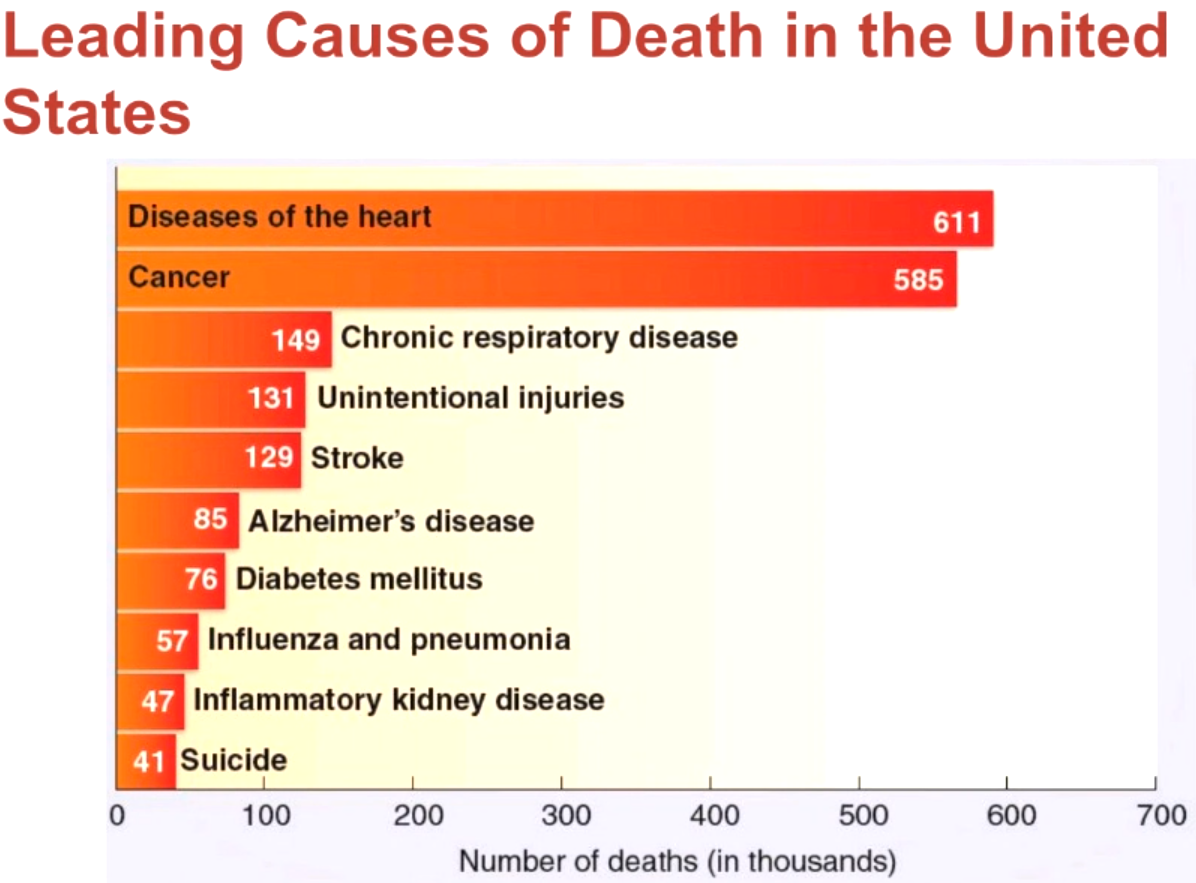
\includegraphics[width=\textwidth]{1_leading_causes_of_death}
	\caption{Leading Causes of Death in the United States}
	\label{fig:leading_causes_of_death_in_us}
\end{figure}

\begin{figure}[H]
	\centering
	\begin{subfigure}[b]{0.475\textwidth}
		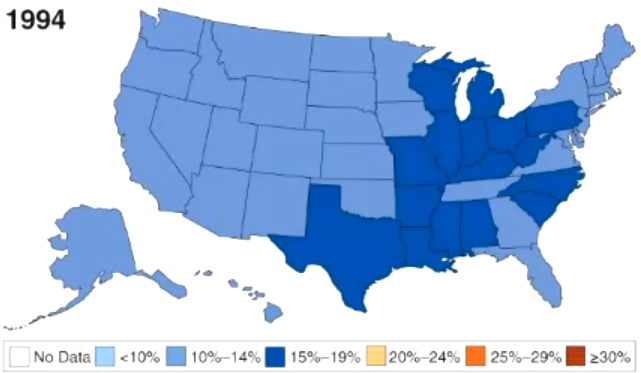
\includegraphics[width=\textwidth]{1_1994_obesity_rates}
		\caption{Obesity rates per U.S. state in 1994.}
		\label{fig:1994_obesity_rates}
	\end{subfigure}
	~
	\begin{subfigure}[b]{0.475\textwidth}
		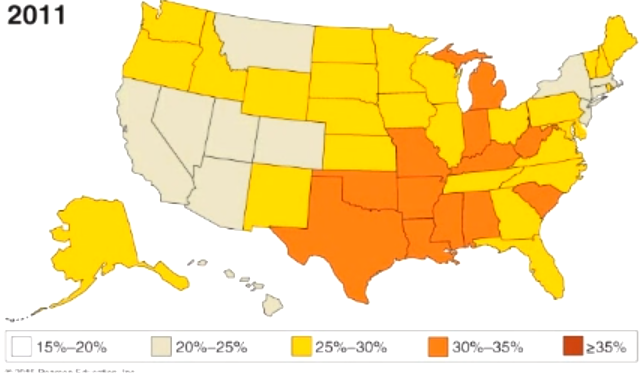
\includegraphics[width=\textwidth]{1_2011_obesity_rates}
		\caption{Obesity rates per U.S. state in 2011.}
		\label{fig:2011_obesity_rates}
	\end{subfigure}
	\caption{A 15-year difference between obesity rates in the United States.}
	\label{fig:15_year_obesity_shift}
\end{figure}

\section{Healthy People 2020}\label{sec:healthy-people-2020}
\begin{itemize}
	\item Nutrition is so important that it has become a national goal
	\item The \emph{Healthy People} plan, revised every decade, identifies goals and objectives to reach by 2020.
\end{itemize}

\subsection{Goals of Healthy People 2020}\label{subsec:goals-of-healthy-people-2020}
\begin{itemize}
	\item Attain high-quality, longer lives free of preventable disease, disability, injury, and premature death
	\item Achieve health equity, eliminate disparities, and improve the health of all groups
	\item Create social and physical environments that promote good health for all
	\item Promote quality of life, healthy development, and healthy behaviors across all life stages
\end{itemize}

\begin{table}[H]
    \centering
    \begin{threeparttable}
		\caption{Weight, Nutrition, and Physical Activity Objecives from \emph{Healthy People 2020}}
		\label{tab:healthy-people-2020}
		\rowcolors{2}{rowmedgreen}{rowlightgreen}
		\begin{tabular}{p{0.35\textwidth} p{0.65\textwidth}}
			\rowcolor{rowdarkgreen}\textbf{Topic} & \textbf{Objective Number and Description}\\
			Weight status & NWS-8. Increase the proportion of adults who are at a healthy weight from 30.8\% to 33.9\%.

			NWS-9. Reduce the proportion of adults who are obese from 34.0\% to 30.6\%.

			NWS-10.2. Reduce the proportion of children aged 6 to 11 years who are considered obese from 17.4\% to 15.7\%.\\
			Food and nutrient composition & NWS-14. Increase the contribution of fruits to the diets of the population aged 2 years and older.

			NWS-15. Increase the variety and contribution of vegetables to the diets of the population aged 2 years and older.\\
			Physical activity & PA--1. Reduce the proportion of adults who engage in no leisure-time physical activity from 36.2\% to 32.6\%.

			PA--2.1. Increase the proportion of adults who engage in aerobic physical activity of at least moderate intensity for at least 150 minutes per week, or 75 minutes per week of vigorous intensity, or an equivalent combination from 43.5\% to 47.9\%.

			PA--2.3. Increase the proportion of adults who perform muscle-strengthening activities on 2 or more days of the week from 21.9\% to 24.1\%.\\
			\rowcolor{rowdarkgreen} & \\
		\end{tabular}
		\begin{tablenotes}
			\small
			\item Data adapted from: \emph{Healthy People 2020 (U.S. Department of Health and Human Services).}
		\end{tablenotes}
	\end{threeparttable}
\end{table}

\section{What Are Nutrients?}\label{sec:what-are-nutrients?}
\begin{itemize}
	\item \definition{Nutrients}{chemicals in foods that are critical to human growth and function}
	\item There are six groups of essential nutrients found in foods:
	\begin{itemize}
		\item \hyperref[subsec:carbohydrates]{Carbohydrates}
		\item \hyperref[subsec:vitamins]{Vitamins}
		\item \hyperref[subsec:fats-and-oils]{Fats and oils}
		\item \hyperref[subsec:minerals]{Minerals}
		\item \hyperref[subsec:proteins]{Proteins}
		\item \hyperref[subsec:water]{Water}
	\end{itemize}
\end{itemize}

\begin{itemize}
	\item \definition{Macronutrients}{nutrients required in relatively large amounts (grams)}
	\begin{itemize}
		\item Provide energy
		\item Carbohydrates, fats and oils, proteins
	\end{itemize}
	\item \definition{Micronutrients}{nutrients required in smaller amounts}
\end{itemize}

\section{Macronutrients Provide Energy}\label{sec:macronutrients-provide-energy}
\begin{itemize}
	\item We measure energy in kilocalories (kcal)\label{dfn:kcal}
	\item \definition{Kilocalorie}{amount of energy required to raise the temperature of 1 kg of water by 1\textdegree{}C}
	\item On food labels, ``Calorie'' actually refers to kilocalories.
\end{itemize}

\textcolor{nutrientgreen}{\subsection{Carbohydrates}\label{subsec:carbohydrates}}
\begin{itemize}
	\item Provide 4 \hyperref[dfn:kcal]{kcal} per gram.
\end{itemize}
\subsubsection{Functions} Primary energy source of fuel for the body, especially for the brain

\subsubsection{Composed of} Chains of carbon, hydrogen, and oxygen

\subsubsection{Best Sources} Whole grains, vegetables, fruits

\textcolor{nutrientorange}{\subsection{Vitamins}\label{subsec:vitamins}}
\subsubsection{Functions} Important source of energy at rest during low-intensity exercise

\subsubsection{Composed of} Carbon, hydrogen, and oxygen

\subsubsection{Best Sources} Vegetable oils, butter and dairy products

\textcolor{nutrientpink}{\subsection{Fats and oils}\label{subsec:fats-and-oils}}
\begin{itemize}
	\item Fats are composed of \hyperref[dfn:lipids]{lipids}, molecules that are insoluble in water
	\item Provide 9 \hyperref[dfn:kcal]{kcal} per gram.
	\item Fats are an important source of fuel for our bodies during times of rest or low-intensity exercise
	\item Our bodies can store fat which can be used for energy while we are not eating
	\item Source of fat-soluble vitamins and essential fatty acids
\end{itemize}
\subsubsection{Functions} Support tissue growth, repair and maintenance

\subsubsection{Composed of} Amino acids made up of carbon, hydrogen, oxygen and nitrogen

\subsubsection{Best Sources} Meats, dairy products, seeds, nuts, legumes

\textcolor{nutrientred}{\subsection{Minerals}\label{subsec:minerals}}
\subsubsection{Functions} Assist with release of macronutrients; critical to building and maintaining bone, muscle, and blood; support immune function and vision

\subsubsection{Composed of} fat-soluble and water-soluble compounds

\subsubsection{Best Sources} fruits, vegetables, dairy products, meats

\textcolor{nutrientpurple}{\subsection{Proteins}\label{subsec:proteins}}
\subsubsection{Functions} Assist with fluid regulation and energy production; maintain health of blood and bones; rid body of harmful by-products of metabolism

\subsubsection{Composed of} Single elements such as sodium, potassium, calcium or iron

\subsubsection{Best Sources} Fruits, vegetables, dairy products, meats

\textcolor{nutrientblue}{\subsection{Water}\label{subsec:water}}
\subsubsection{Functions} Ensures proper fluid balance; assists in regulation of nerve impulses, body temperature, and muscle contractions

\subsubsection{Composed of} Hydrogen and oxygen

\subsubsection{Best Sources} Water, juices, soups, fruits, vegetables
% Stopped at 25:29

\end{document}